% main.tex - The Master Document File
% This file provides the high-level structure of the document.

% Load all packages, settings, and custom commands from the preamble file.
% preamble.tex - Packages and Document Configuration
% FIX: Added command to remove paragraph indentation globally.

\documentclass[12pt, a4paper, oneside]{scrreprt} % Using KOMA-Script for better typography

% --- GEOMETRY & SPACING ---
\usepackage[a4paper, margin=1in]{geometry}
\usepackage{setspace}
\setstretch{1.5}
\setlength{\parskip}{6pt} % Space between paragraphs
\setlength{\parindent}{0pt} % Removes the indentation from the start of paragraphs
\usepackage{microtype} % Improves justification and spacing

% --- FONTS & ENCODING ---
\usepackage[utf8]{inputenc}
\usepackage[T1]{fontenc}

% --- GRAPHICS, TABLES, & FIGURES ---
\usepackage{graphicx}
\usepackage{amssymb} % Defines the \square symbol for the appendix
\usepackage{booktabs} % For professional tables
\usepackage{longtable}
\usepackage{caption}
\usepackage{float}
\usepackage{pgfplots}
\pgfplotsset{compat=1.18}
\usepackage{tabularx}
\newcolumntype{Y}{>{\raggedright\arraybackslash}X} % Custom column type

% --- HEADERS & FOOTERS ---
\usepackage{fancyhdr}
\pagestyle{fancy}
\fancyhf{} % Clear all header and footer fields
\fancyhead[L]{\nouppercase{\leftmark}}
\fancyfoot[C]{\thepage}
\renewcommand{\headrulewidth}{0.4pt}
\renewcommand{\footrulewidth}{0pt}

% --- BIBLIOGRAPHY (BibLaTeX with IEEE Style) ---
\usepackage[style=ieee, backend=biber, sorting=none]{biblatex}
\addbibresource{references.bib} % The .bib file

% --- HYPERLINKS & METADATA ---
\usepackage[colorlinks=true, linkcolor=black, urlcolor=blue, citecolor=black]{hyperref}
\hypersetup{
    pdfauthor={Jane Doe}, % Anonymized
    pdftitle={Assessment of the Impact of Solid Waste Disposal on Public Health (Portfolio Sample)},
    pdfsubject={Undergraduate Thesis Portfolio Sample}
}

% --- OTHER UTILITIES ---
\usepackage{enumitem} % For customizing lists



\begin{document}

% --- FRONT MATTER ---
% This section includes the title page, declaration, abstract, etc.
% Page numbers are in Roman numerals.
%\frontmatter
\pagestyle{empty} % No headers/footers on initial front matter pages

% frontmatter/00_titlepage.tex
% FIX: Anonymized all university, department, and location details with placeholders.
% This makes the file a reusable and professional portfolio template.
% FIX: Further reduced vertical spacing to guarantee the content fits on a single page.

\begin{titlepage}
\centering
\vspace*{0.5cm}

{\huge\bfseries [Your University Name]}\\[0.8cm]

% --- Placeholder for University Logo ---
% In a real project, you would place the university logo here.
% Example: \includegraphics[width=0.25\textwidth]{path/to/your/logo.png}
\framebox(100,100){Logo Placeholder}\\[1cm]

{\Large\bfseries [College Name]}\\[4pt]
{\Large\bfseries [Department Name]}\\[1.2cm]

{\LARGE\bfseries Assessment of the Impact of Solid Waste Disposal on Public Health:}\\[8pt]
{\LARGE\bfseries A Case Study of a Peri-Urban Dumpsite}\\[1.5cm]

{\large\bfseries By:}\\[4pt]
{\large [Your Name]}\\[4pt]
{\large ID NUMBER: [ID Number]}\\[1.2cm]

A Thesis Submitted to the [Department Name], [College Name], [Your University Name], in Partial Fulfillment of the Requirements for the Degree of [Degree Name]\\[1.2cm]

{\large\bfseries Advisor:} [Your Advisor's Name]\\[1.5cm]

\vfill % This command pushes the following content to the bottom of the page

{\large [Date of Submission]}\\[8pt]


\end{titlepage}


\clearpage
% frontmatter/01_declaration.tex

\thispagestyle{empty} % No header or footer on this page
\noindent\textbf{Declaration}\\[1em]
I declare that this thesis is my original work and has not been submitted for a degree in any other university.\\[3em]
\noindent\rule{0.5\linewidth}{0.4pt}\\
Jane Doe \hfill Date: \rule{0.25\linewidth}{0.4pt}

\vfill

\noindent\textbf{Approval}\\[1em]
This thesis has been submitted for examination with my approval as university advisor.\\[3em]
\noindent\rule{0.5\linewidth}{0.4pt}\\
Dr.~John Smith (Advisor) \hfill Date: \rule{0.25\linewidth}{0.4pt}

\clearpage

\pagestyle{fancy} % Re-enable professional headers/footers for the rest
% frontmatter/02_abstract_acronyms.tex

\chapter*{Abstract}
\addcontentsline{toc}{chapter}{Abstract}
This study assesses the public health impacts associated with an open dumpsite in a peri-urban town in Ethiopia. A mixed-methods cross-sectional design was used, combining a household survey with key informant interviews and systematic site observations. Quantitative analysis summarized prevalence of respiratory, gastrointestinal, and dermatological conditions and tested associations with residential proximity to the dumpsite; qualitative analysis explored community perceptions and institutional challenges. Findings indicate elevated self-reported rates of respiratory and gastrointestinal illness among households nearer the site and strong perceived links between open dumping, burning, and health. The study recommends targeted risk communication, improved collection and segregation, engineered sanitary disposal, and integration of informal waste workers into safer systems. The results provide evidence for local policy and practical interventions to reduce exposure and disease burden.

\vspace{2em}
\noindent\textbf{Keywords:} Solid Waste Management, Public Health, Dumpsites, Environmental Health, Urban Planning, Ethiopia

\clearpage

\chapter*{Acronyms and Abbreviations}
\addcontentsline{toc}{chapter}{Acronyms and Abbreviations}
\begin{tabularx}{0.8\textwidth}{@{} l Y @{}}
\toprule
\textbf{SWM} & Solid Waste Management\\
\textbf{MSW} & Municipal Solid Waste\\
\textbf{ISWM} & Integrated Solid Waste Management\\
\textbf{ITCZ} & Inter-Tropical Convergence Zone\\
\textbf{WHO} & World Health Organization\\
\textbf{EPA} & Environmental Protection Authority (Ethiopia)\\
\textbf{FMoH} & Federal Ministry of Health (Ethiopia)\\
\textbf{SPSS} & Statistical Package for the Social Sciences\\
\bottomrule
\end{tabularx}

\clearpage
% frontmatter/03_acknowledgements.tex

\chapter*{Acknowledgements}
\addcontentsline{toc}{chapter}{Acknowledgements}
The author wishes to express sincere gratitude to the Department of Biology at Mekelle University for providing the academic foundation for this research. Special thanks are extended to my advisor, Dr.~John Smith, for his invaluable supervision, guidance, and encouragement throughout this project.

I am also grateful to the municipal officials and health officers in the study area for their cooperation and for providing access to essential data.

Finally, my deepest appreciation goes to the community members and residents who generously gave their time to participate in the surveys and interviews. Their insights were central to the success of this study.

\clearpage

% --- TABLE OF CONTENTS & LISTS ---
% Automatically generate the Table of Contents, List of Tables, and List of Figures.
\tableofcontents
\clearpage
\listoftables
\clearpage
\listoffigures
\clearpage

% --- MAIN CONTENT ---
% This is the body of the thesis, with chapters imported from separate files.
% Switches to Arabic numerals for page numbers.
%\mainmatter
\pagestyle{fancy}

% chapters/01_introduction.tex

\chapter{Introduction}
\label{chap:introduction}

\section{Background of the Study}
\label{sec:background}
Solid waste management (SWM) remains one of the most pressing environmental and public health challenges in the 21st century, particularly in low- and middle-income countries experiencing rapid urbanization, population growth, and industrial expansion \cite{Kaza2018, Wilson2015}. Inadequate waste collection services, limited infrastructure, and poor enforcement of waste disposal regulations often result in practices such as open dumping, indiscriminate littering, and uncontrolled burning of solid waste. These practices contribute not only to environmental degradation—through air, water, and soil contamination—but also pose significant health risks to nearby populations due to the proliferation of vectors, exposure to hazardous substances, and respiratory problems caused by smoke and pollutants \cite{UNEP2015, Ferronato2019}.

In the African context, urban waste generation is growing at an alarming rate, outstripping the institutional and financial capacities of local governments to manage it effectively \cite{Hoornweg2012}. Ethiopia exemplifies this struggle, where urban solid waste management systems are often underfunded, poorly planned, and lack community participation. A study by Alemayehu et al. \cite{Alemayehu2021} highlighted that in many Ethiopian cities, less than 50\% of the generated waste is properly collected and managed, with the remainder either openly dumped or burned. The resulting health consequences include increased prevalence of respiratory illnesses, vector-borne diseases such as malaria and dengue, and gastrointestinal infections due to water contamination.

This study focuses on a representative peri-urban town in northern Ethiopia, which typifies this growing urban challenge. The town’s main waste disposal site operates as an open dump, lacking any engineered containment or environmental safeguards. Situated near residential areas, the site poses direct and indirect health risks to local communities, including children, the elderly, and waste pickers. Local observations and anecdotal evidence suggest a rise in respiratory issues, skin infections, and gastrointestinal diseases among the nearby population. However, there has been limited systematic research to assess the scale and nature of the public health impact resulting from this unmanaged waste site. This study aims to fill that gap.

\section{Statement of the Problem}
Solid waste management (SWM) in Ethiopia faces critical challenges due to rapid urbanization and limited infrastructure. Most urban areas rely on open dumping and burning, which leads to environmental pollution and increased public health risks. Poorly managed waste attracts disease vectors, emits toxic gases, and produces leachate that contaminates water sources, resulting in illnesses such as respiratory infections, waterborne diseases, and skin conditions \cite{MoUDC2017, WHO2018}.

While larger cities have received some attention, smaller towns remain under-researched. The study area exemplifies this issue. Its main disposal site is an open, unregulated dump that receives mixed, unsorted waste. The site lacks basic containment or safety measures, and open burning is common. Residents living nearby are exposed to air and water pollution, with informal reports suggesting a high prevalence of related illnesses. Despite clear health concerns, no systematic study had assessed the specific public health impacts. This lack of data limits the ability of local authorities to respond effectively.

\section{Objectives}
\subsection{General Objective}
The main objective of the study was to assess the impact of solid waste disposal practices at the local dumpsite on the public health of nearby communities, with the aim of generating evidence to support targeted environmental and health interventions.

\subsection{Specific Objectives}
\begin{enumerate}
    \item To examine the existing solid waste management system in the town, with an emphasis on disposal practices at the site.
    \item To identify and quantify the prevalence of key health conditions—such as respiratory, gastrointestinal, and dermatological illnesses—among residents living near the site.
    \item To assess community perceptions regarding the health impacts of living near the waste disposal site.
\end{enumerate}

\section{Research Questions}
\begin{enumerate}[label=\arabic*.]
    \item What were the solid waste disposal practices at the site, and how did they align with national and international public health standards?
    \item What were the most prevalent health issues reported by residents living in proximity to the waste site?
    \item Was there a statistically significant relationship between household proximity to the site and the incidence of specific health conditions?
\end{enumerate}

\section{Hypotheses}
\begin{enumerate}[label=H\arabic*.]
    \item The solid waste disposal practices at the site were environmentally inadequate and posed health risks to surrounding communities.
    \item Residents living closer to the site experienced a higher prevalence of respiratory, gastrointestinal, and dermatological conditions compared to those living farther away.
    \item The majority of community members living near the site perceived a direct connection between the waste disposal site and their family’s health issues.
\end{enumerate}

\section{Significance of the Study}
This study generates critical evidence to inform urban planning and public health policy. By assessing the health impacts of solid waste disposal practices, the research supports the development of more sustainable waste management systems and interventions aimed at reducing community exposure to environmental health risks. For public health authorities, the findings can guide the design of effective health education campaigns, strengthen disease surveillance, and enhance risk communication. Academically, the study contributes to the limited literature on environmental health in secondary towns of developing countries.

\section{Expected Output}
The research produced a comprehensive assessment of the public health impacts associated with the solid waste disposal practices at the local site. By generating both quantitative and qualitative data, the study identified operational deficiencies in waste management and quantified the prevalence of key health conditions. The analysis determined whether a statistically significant relationship existed between proximity to the site and adverse health outcomes. Based on these findings, the study provides actionable, context-specific policy recommendations to improve waste management and reduce public health risks.

% chapters/02_literature_review.tex

\chapter{Literature Review}
\label{chap:literature_review}

\section{Global Perspectives on Solid Waste Disposal and Health Impacts}
Globally, municipal solid waste (MSW) generation was expected to reach approximately 3.4 billion tonnes annually by 2050, with the most rapid increases occurring in low- and middle-income countries \cite{Kaza2018}. In many of these regions, over 90\% of waste was disposed of in open dumps or uncontrolled landfills, often without adequate environmental safeguards. Such practices led to the proliferation of disease vectors, emission of toxic gases from burning, and contamination of water sources by leachate, all of which contributed to adverse health outcomes. Studies worldwide linked exposure to poorly managed waste sites to respiratory illnesses caused by air pollutants, gastrointestinal infections from contaminated water, dermatological conditions, and vector-borne diseases such as malaria and dengue \cite{Porta2009, Ferronato2019}.

Integrated Solid Waste Management (ISWM) is widely recognized as an effective strategy for mitigating these risks. ISWM emphasizes waste minimization through reduction, reuse, and recycling, combined with environmentally safe disposal methods \cite{UNEP2015}. However, many low- and middle-income countries face challenges in implementing ISWM due to financial constraints, lack of technical expertise, and weak institutional frameworks.

\section{Solid Waste Management in Ethiopia}
Ethiopia’s rapidly expanding urban population has intensified the challenges of SWM. A substantial portion of municipal waste remains uncollected or is disposed of improperly through open dumping and burning, particularly in rapidly growing cities \cite{Gebremedhin2018}. Research in Addis Ababa and Hawassa highlighted significant health risks among residents and informal waste pickers, including elevated cases of respiratory ailments, diarrheal diseases, and skin infections \cite{Bogale2019, Abebe2018}. The 2017 collapse of the Koshe landfill in Addis Ababa, which claimed over 100 lives, starkly underscored the urgent need for improved systems.

Systemic barriers hinder effective SWM in Ethiopia, including inadequate funding, limited technical capacity, low public awareness, and weak enforcement of environmental regulations \cite{WorldBank2018}. These obstacles contribute to unsafe practices, resulting in environmental contamination and increased health hazards \cite{UNEP2018}.

\section{Health Impacts of Open Dumpsites}
Open dumpsites pose major public health risks. Airborne pollutants such as methane and hydrogen sulfide, emitted from decomposing waste, can cause respiratory illnesses including asthma and chronic bronchitis \cite{Ferronato2019, Ndejjo2016}. Surface and groundwater contamination from leachate can cause gastrointestinal infections and other waterborne diseases \cite{Porta2009, WHO2018}.

Furthermore, open dumps are breeding sites for flies, mosquitoes, and rodents, which transmit diseases such as malaria, dengue fever, and leptospirosis \cite{Wilson2015, Bogale2019}. Skin conditions are also common among residents and informal waste pickers who come into direct contact with waste materials \cite{Abebe2018}. These impacts reduce quality of life and impose economic burdens through increased healthcare costs and lost productivity.

\section{Community Perception and Public Participation}
Community perception plays a crucial role in the success of SWM initiatives. Residents near dumpsites often associate poor waste disposal with health risks, although awareness of specific causes and preventive measures can be limited \cite{Kibreab2020}. Understanding these perceptions is important for designing public health campaigns that resonate with local experiences.

Public participation is a key pillar of sustainable SWM. In Ethiopia, however, engagement often remains low due to lack of education, insufficient incentives, and weak institutional support \cite{Gebremedhin2018}. Encouraging active involvement through education and empowerment of local stakeholders can improve waste sorting at source, reduce illegal dumping, and promote recycling.

\section{SWM Policy and Institutional Framework in Ethiopia}
Ethiopia has developed several policies to improve SWM. The Environmental Policy \cite{EPA2017} and Urban Sanitation and Hygiene Strategy \cite{FMoH2016} emphasize integrated approaches, promoting waste reduction, recycling, and safe disposal. Responsibilities are distributed across federal, regional, and local levels, with municipalities central in collection and disposal \cite{WorldBank2018}.

Despite these frameworks, gaps persist due to inadequate coordination, limited resources, and weak enforcement \cite{Gebremedhin2018}. The informal sector, which provides livelihoods for many, is often overlooked, resulting in missed opportunities for inclusive management.

\input{chapters/03_methods.tex}
% chapters/04_results.tex
% Presents the quantitative and qualitative findings of the study.
% FIX: Corrected pgfplots syntax to handle special characters in labels.
% FIX: Restored the third figure which was accidentally deleted.

\chapter{Data Presentation and Analysis}
\label{chap:results}

This chapter presents the findings of the study based on quantitative household survey data, qualitative interviews with key informants, and field observations at the Beadu solid waste disposal site. The analysis highlights socio-demographic characteristics, prevalence of reported health problems, waste management practices, perceived health impacts, and community awareness.

\section{Socio-Demographic Characteristics of Respondents}

A total of 150 households were surveyed. Table~\ref{tab:demographics} summarizes the socio-demographic characteristics of the respondents. The majority of respondents were female (64.7\%), reflecting their central role in household management and caregiving. The dominant age group was 31--45 years (43.3\%). Educational attainment was low, with 60\% of respondents having no formal or only primary education. Regarding occupation, informal employment (36.7\%) and unemployment (26.7\%) were most common. Nearly half of respondents (46.7\%) lived within 500 meters of the Beadu site, indicating high potential exposure.

\begin{table}[h!]
\centering
\caption{Socio-Demographic Characteristics of Surveyed Households (N=150)}
\label{tab:demographics}
\begin{tabular}{@{}llcc@{}}
\toprule
\textbf{Characteristic} & \textbf{Category} & \textbf{Frequency (n)} & \textbf{Percentage (\%)} \\ \midrule
Gender of Respondent & Male & 53 & 35.3 \\
                     & Female & 97 & 64.7 \\ \midrule
Age Group (Years)    & 18--30 & 30 & 20.0 \\
                     & 31--45 & 65 & 43.3 \\
                     & 46--60 & 40 & 26.7 \\
                     & >60    & 15 & 10.0 \\ \midrule
Education Level       & No formal education & 45 & 30.0 \\
                      & Primary education    & 45 & 30.0 \\
                      & Secondary education  & 35 & 23.3 \\
                      & Tertiary education   & 25 & 16.7 \\ \midrule
Occupation            & Employed (Formal)    & 30 & 20.0 \\
                      & Employed (Informal)  & 55 & 36.7 \\
                      & Unemployed           & 40 & 26.7 \\
                      & Housewife/Student/Other & 25 & 16.7 \\ \midrule
Distance from Site & <500 meters & 70 & 46.7 \\
                   & 500m--1 km  & 80 & 53.3 \\ \bottomrule
\end{tabular}
\end{table}


\section{Prevalence of Reported Health Conditions}

Respondents reported a range of health problems over the previous six months. The most frequently reported conditions were acute respiratory infections (63.3\%), diarrheal diseases (53.3\%), and skin irritations (46.7\%). Table~\ref{tab:health} and Figure~\ref{fig:healthproblems} present the distribution.

\begin{table}[h!]
\centering
\caption{Self-reported health problems among surveyed households (N=150).}
\label{tab:health}
\begin{tabular}{@{}lcc@{}}
\toprule
\textbf{Health Problem} & \textbf{n} & \textbf{Percentage (\%)} \\ 
\midrule
Acute Respiratory Infections (ARIs) & 95 & 63.3 \\
Diarrheal Diseases                   & 80 & 53.3 \\
Skin Rashes/Irritations              & 70 & 46.7 \\
Eye Irritations                      & 55 & 36.7 \\
Malaria/Vector-borne Diseases        & 30 & 20.0 \\
Other (e.g., headaches, nausea)      & 25 & 16.7 \\
\bottomrule
\end{tabular}
\end{table}

\begin{figure}[h!]
\centering
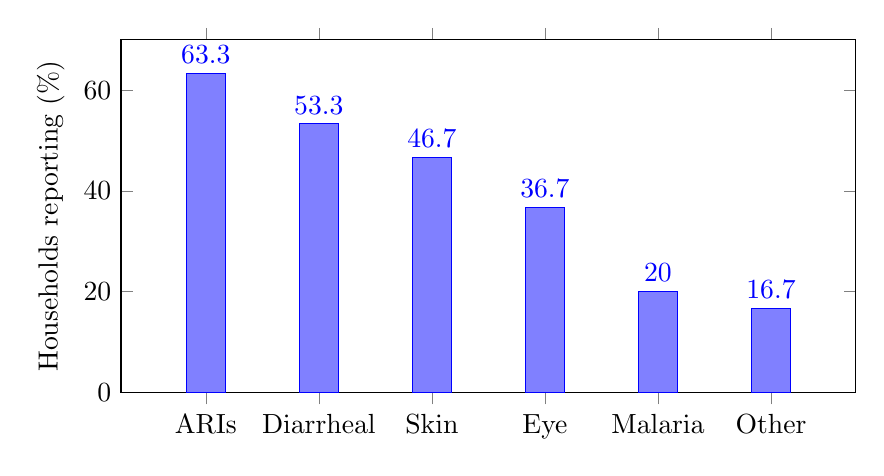
\begin{tikzpicture}
\begin{axis}[
    ybar,
    bar width=14pt,
    width=0.9\textwidth,
    height=0.5\textwidth,
    ymin=0,
    ymax=70,
    ylabel={Households reporting (\%)},
    symbolic x coords={ARIs, Diarrheal, Skin, Eye, Malaria, Other},
    xtick=data,
    nodes near coords,
    nodes near coords align={vertical},
    enlarge x limits=0.15,
]
\addplot+[fill=blue!50] coordinates {(ARIs,63.3) (Diarrheal,53.3) (Skin,46.7) (Eye,36.7) (Malaria,20.0) (Other,16.7)};
\end{axis}
\end{tikzpicture}
\caption{Prevalence of self-reported health problems among households.}
\label{fig:healthproblems}
\end{figure}


\section{Association Between Proximity and Reported Illnesses}

A chi-square test revealed a statistically significant association between proximity to the Beadu site and perceived health problems ($\chi^2(1)=5.21, p<0.05$). Table~\ref{tab:proximity} shows that households closer to the site (<500 meters) were far more likely (92.9\%) to link their illnesses to the dumpsite than those living farther away. This is visualized in Figure~\ref{fig:proximity}.

\begin{table}[h!]
\centering
\caption{Perceived link between proximity to site and health problems (N=150).}
\label{tab:proximity}
\begin{tabular}{@{}lccc@{}}
\toprule
\textbf{Proximity to Site} & \textbf{Yes (n,\%)} & \textbf{No (n,\%)} & \textbf{Total} \\ 
\midrule
< 500 meters   & 65 (92.9) & 5 (7.1)   & 70 \\
500m--1 km     & 63 (78.8) & 17 (21.2) & 80 \\
\midrule
Total          & 128 (85.3) & 22 (14.7) & 150 \\
\bottomrule
\end{tabular}
\end{table}

\begin{figure}[h!]
\centering
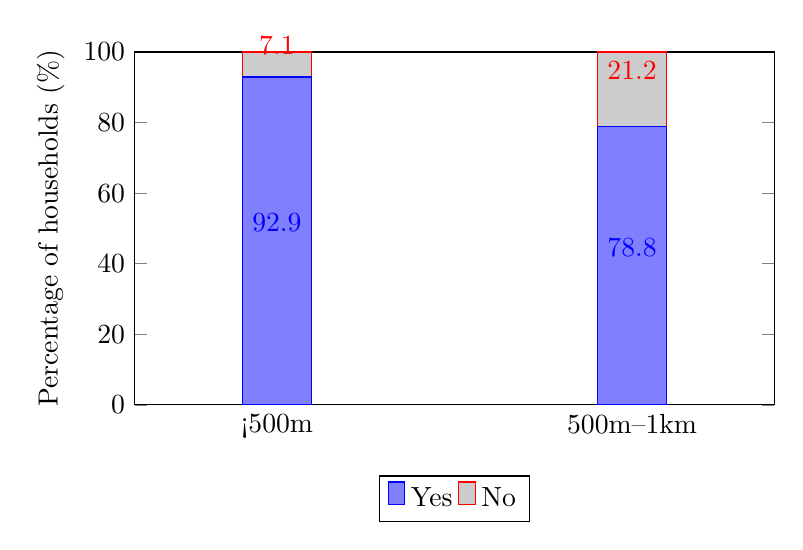
\begin{tikzpicture}
\begin{axis}[
    ybar stacked,
    bar width=25pt,
    width=0.8\textwidth,
    height=0.5\textwidth,
    ymin=0,
    ymax=100,
    ylabel={Percentage of households (\%)},
    symbolic x coords={groupA, groupB}, % Use simple internal names
    xtick=data,
    xticklabels={<500m, 500m--1km}, % Provide the display text here
    nodes near coords,
    nodes near coords align={vertical},
    enlarge x limits=0.4,
    legend style={at={(0.5,-0.2)},anchor=north,legend columns=-1},
]
\addplot+[fill=blue!50] coordinates {(groupA,92.9) (groupB,78.8)};
\addplot+[fill=gray!40] coordinates {(groupA,7.1) (groupB,21.2)};
\legend{Yes, No}
\end{axis}
\end{tikzpicture}
\caption{Perceived link between proximity to site and health problems.}
\label{fig:proximity}
\end{figure}


\section{Community Awareness and Attitudes}

Awareness of health risks was generally high (78\% of respondents agreed that improper waste disposal causes illness). However, satisfaction with municipal waste services was very low (78\% disagreed that services were adequate). While 45\% expressed willingness to pay for improved services, actual segregation practices remained minimal (only 25\% practiced separation at home). Table~\ref{tab:awareness} and Figure~\ref{fig:awareness} summarize these attitudes.

\begin{table}[h!]
\centering
\caption{Community awareness and attitudes towards solid waste management.}
\label{tab:awareness}
\begin{tabular}{@{}lccc@{}}
\toprule
\textbf{Statement} & \textbf{Agree (\%)} & \textbf{Neutral (\%)} & \textbf{Disagree (\%)} \\ 
\midrule
Improper waste disposal causes health problems & 78.0 & 15.0 & 7.0 \\
Municipal waste collection is adequate          & 12.0 & 10.0 & 78.0 \\
I segregate waste at home                       & 25.0 & 18.0 & 57.0 \\
I am willing to pay more for better SWM services& 45.0 & 30.0 & 25.0 \\
Public health education on waste is sufficient  & 10.0 & 15.0 & 75.0 \\
\bottomrule
\end{tabular}
\end{table}

\begin{figure}[h!]
\centering
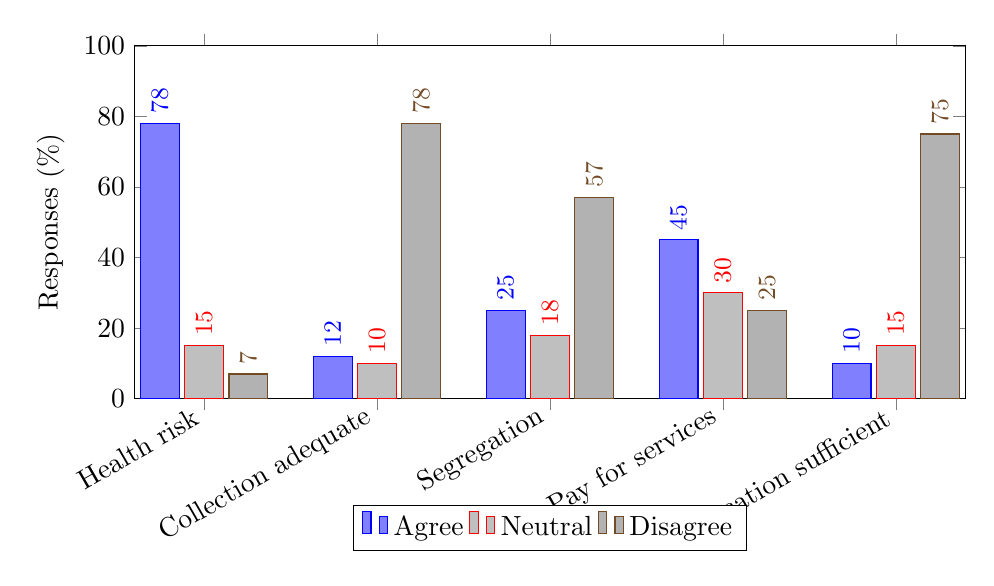
\begin{tikzpicture}
\begin{axis}[
    ybar,
    bar width=14pt,
    width=\textwidth,
    height=0.5\textwidth,
    ymin=0,
    ymax=100,
    ylabel={Responses (\%)},
    symbolic x coords={Health risk, Collection adequate, Segregation, Pay for services, Education sufficient},
    xtick=data,
    x tick label style={rotate=30, anchor=east},
    nodes near coords,
    nodes near coords style={font=\small, rotate=90, anchor=west},
    enlarge x limits=0.1,
    legend style={at={(0.5,-0.3)},anchor=north,legend columns=-1},
]
\addplot+[fill=blue!50] coordinates {(Health risk,78) (Collection adequate,12) (Segregation,25) (Pay for services,45) (Education sufficient,10)};
\addplot+[fill=gray!50] coordinates {(Health risk,15) (Collection adequate,10) (Segregation,18) (Pay for services,30) (Education sufficient,15)};
\addplot+[fill=black!30] coordinates {(Health risk,7) (Collection adequate,78) (Segregation,57) (Pay for services,25) (Education sufficient,75)};
\legend{Agree, Neutral, Disagree}
\end{axis}
\end{tikzpicture}
\caption{Community awareness and attitudes towards solid waste management.}
\label{fig:awareness}
\end{figure}


% chapters/05_discussion.tex
% This chapter provides an in-depth discussion of the research findings.

\chapter{Discussion}
\label{chap:discussion}

This chapter interprets the findings presented in Chapter 4, contextualizing them within existing academic literature and theoretical frameworks. It also explores the public health and policy implications of the results.

\section{Comparison with Prior Studies}
The conditions at the study site exemplify the challenges typical of open dumping in developing countries. The high prevalence of self-reported respiratory infections (63.3\%) is consistent with studies in other parts of Africa that have linked proximity to dumpsites with increased rates of respiratory and gastrointestinal diseases \cite{Ndejjo2016}. The observed practice of open waste burning is a known source of particulate matter and toxic gases, corroborating global evidence on the health risks of uncontrolled combustion \cite{Porta2009}.

Similarly, the high prevalence of diarrheal diseases (53.3\%) aligns with literature that links groundwater contamination by leachate to waterborne illnesses \cite{Ferronato2019}. The observed presence of vectors like flies and rodents reinforces findings from studies at other major Ethiopian dumpsites, such as Koshe and Hawassa, where vector proliferation was also identified as a significant health hazard \cite{Bogale2019, Abebe2018}.

The strong perception (85.3\%) among residents that the dumpsite negatively affects their health mirrors the Environmental Health Paradigm, which posits that communities often directly recognize environmental stressors as key determinants of their well-being. This validates the Exposure Pathway Model in this context: inhalation (of smoke and dust), ingestion (of contaminated water or food), dermal contact, and vector bites all emerged as plausible routes of exposure according to both observations and community reports.

\section{Implications for Public Health and SWM}
The findings highlight several urgent health and policy challenges:
\begin{itemize}
    \item \textbf{Public Health Burden:} The dominance of Acute Respiratory Infections (ARIs) and diarrheal diseases suggests ongoing community exposure to air and water contamination originating from the dumpsite. It is likely that seasonal variations exacerbate these risks, with increased dust and burning during the dry season and wider leachate spread during rainy months.
    
    \item \textbf{Community Perceptions vs. Practice:} The strong awareness of health risks contrasts sharply with the low rate of household waste segregation. This indicates a significant gap between knowledge and practice, likely driven by the lack of reliable municipal collection infrastructure and incentives for segregation.
    
    \item \textbf{Institutional Gaps:} The absence of basic engineering controls (such as liners, leachate management systems, or gas vents) at the site magnifies the environmental and health risks. Furthermore, the practice of informal scavenging, while providing a livelihood for some, perpetuates cycles of exposure and contributes to the dispersal of waste into the surrounding environment.
    
    \item \textbf{Financing Opportunities:} The finding that nearly half of the respondents expressed a willingness to pay for better services suggests a potential avenue for developing sustainable funding mechanisms for SWM, provided such systems are implemented with transparency and accountability.
\end{itemize}

Overall, the results reinforce the global consensus on the dangers of open dumping while illustrating the acute local realities in the study area. The evidence strongly supports the need for integrated waste management reforms, enhanced public health education, and institutional strengthening.


% chapters/07_conclusions_recommendations.tex
% This corresponds to the "conclusions and recommendations" chapter you requested.

\chapter{Conclusions and Recommendations}
\label{chap:conclusions}

This chapter presents the main conclusions derived from the study and outlines practical recommendations for addressing the identified public health and environmental risks associated with the local dumpsite. The conclusions synthesize the key findings, while the recommendations are targeted toward policymakers, municipal authorities, public health institutions, and the community.

\section{Conclusions}
The findings of this study clearly demonstrate that the solid waste disposal site poses significant risks to both the environment and the health of surrounding communities. Several major conclusions can be drawn:

\begin{enumerate}
    \item The current operational practices at the dumpsite—characterized by uncontrolled open dumping, frequent burning of waste, and an absence of engineering controls—create multiple pathways for human exposure to contaminants. These include air pollution from smoke and dust, proliferation of disease vectors such as flies and rodents, and potential contamination of surface and groundwater by leachate.

    \item Adverse health impacts are strongly reflected in the community survey data. Households residing in closer proximity to the dumpsite reported substantially higher rates of respiratory illnesses and gastrointestinal conditions. This statistically significant association indicates that inadequate solid waste management is a direct contributor to heightened health vulnerability in the community.

    \item While community awareness of the health risks associated with improper waste disposal is relatively high, this knowledge does not translate into safer household practices like waste segregation. This gap is primarily due to the lack of adequate municipal waste collection services and supporting infrastructure.

    \item Systemic institutional limitations, including insufficient municipal capacity, budgetary constraints, and weak enforcement of existing solid waste management policies, are root causes that perpetuate the problem.
\end{enumerate}

\section{Recommendations}
To mitigate the adverse health and environmental impacts, the following recommendations are proposed, addressing short-term, medium-term, and long-term actions:

\begin{itemize}
    \item \textbf{Implement Immediate Risk Reduction Measures:} Municipal authorities should immediately prohibit the open burning of waste. Access to the dumpsite should be controlled to limit unsafe scavenging activities, especially by vulnerable populations.

    \item \textbf{Improve Waste Collection and Introduce Segregation:} Expanding the coverage, frequency, and reliability of municipal waste collection services is critical. In parallel, the municipality should launch a pilot program for source segregation to reduce the volume of waste sent to the dumpsite.

    \item \textbf{Transition Towards Engineered Disposal Systems:} A phased, long-term plan should be developed to upgrade the site to a controlled or sanitary landfill. Initial steps should include the application of daily soil cover, followed by future implementation of leachate collection systems.

    \item \textbf{Protect and Integrate Informal Waste Workers:} Informal waste pickers should be formally recognized and integrated into the waste management system. Providing training on health and safety and ensuring access to personal protective equipment (PPE) is essential.

    \item \textbf{Strengthen Public Health Interventions:} Local health authorities should intensify disease surveillance in neighborhoods near the dumpsite. Community-based health education campaigns should be expanded to promote hygienic practices and raise awareness about exposure pathways.
\end{itemize}


% chapters/08_action_plan_budget.tex
% This corresponds to the "action plan and budget" chapter you requested.

\chapter{Action Plan and Budget}
\label{chap:action_plan}

This chapter outlines the original timeline and a conceptual budget framework for the research project, as presented in the proposal stage.

\section{Time Table of the Study}
The study was planned and executed according to the schedule presented in Table \ref{tab:timetable}. This timeline ensured that all phases, from proposal refinement to final defense, were completed systematically.

\begin{table}[H]
    \centering
    \caption{Original time table of the study.}
    \label{tab:timetable}
    \begin{tabular}{@{}cll@{}}
    \toprule
    \textbf{No} & \textbf{Action / Objective} & \textbf{Date} \\ \midrule
    1 & Refining research proposal & March 2017 \\
    2 & Submission of final proposal & April 2017 \\
    3 & Proposal defense & May 2017 \\
    4 & Field survey and site selection & June 2017 \\
    5 & Finalizing data collection tools & June 2017 \\
    6 & Household and informant interviews & July 2017 \\
    7 & Data collection period & July--October 2017 \\
    8 & Data entry and analysis & November 2017 \\
    9 & Writing initial report draft & December 2017 \\
    10 & Submission of first draft of thesis & January 2018 \\
    11 & Final thesis defense & June 2018 \\ \bottomrule
    \end{tabular}
\end{table}

\section{Expense of the Research (Budget Breakdown)}
The budget for this research was designed to cover all necessary expenses from personnel to materials. Table \ref{tab:budget} provides a breakdown of the required financial resources. This structure is intended as a template for future research projects of a similar scale.

\begin{table}[H]
    \centering
    \caption{Conceptual budget breakdown for the research project.}
    \label{tab:budget}
    \begin{tabularx}{\textwidth}{@{}lX@{}}
    \toprule
    \textbf{S.No.} & \textbf{Items and Description} \\ \midrule
    1 & \textbf{Personnel:} Honoraria for the major advisor, stipends for field assistants and data enumerators. \\
    2 & \textbf{Transportation:} Local travel costs for the research team to and from the study site and for survey administration. \\
    3 & \textbf{Stationery and Printing:} Costs for printing questionnaires, consent forms, reports, and purchasing necessary stationery. \\
    4 & \textbf{Equipment:} Rental or purchase of a digital camera for site documentation and an audio recorder for interviews. \\
    5 & \textbf{Field Materials:} Purchase of personal protective equipment (masks, gloves) for the research team during site visits. \\
    6 & \textbf{Data Analysis:} Costs associated with statistical software licenses or consultation, if required. \\
    7 & \textbf{Miscellaneous:} A small fund for unforeseen expenses during fieldwork. \\ \midrule
    & \textbf{Sub Total:} \rule{0.25\linewidth}{0.4pt} \\
    & \textbf{Contingency (10\%):} \rule{0.25\linewidth}{0.4pt} \\
    & \textbf{Grand Total:} \rule{0.25\linewidth}{0.4pt} \\ \bottomrule
    \end{tabularx}
\end{table}



\clearpage
% Print the bibliography, titled "References".
% The citations are managed by BibLaTeX from the 'references.bib' file.
\printbibliography[title={References}]

% --- APPENDICES & BIBLIOGRAPHY ---
% This section includes supplementary materials and the bibliography.
\appendix
\pagestyle{fancy}
% backmatter/appendix_questionnaire.tex
% This appendix contains the sample questionnaire used for the household survey.

\chapter{Sample Household Survey Questionnaire}
\label{app:questionnaire}

\textbf{Questionnaire ID:} \hrulefill \hspace{1cm}
\textbf{Date of Interview:} \hrulefill \\[1em]

\section*{Section 1: Socio-Demographic Information}

\begin{enumerate}[label=\arabic*.]
    \item Gender of Respondent:
    \begin{itemize}
        \item[$\square$] Male
        \item[$\square$] Female
    \end{itemize}

    \item Age of Respondent (Years): \hrulefill

    \item Household Size (Number of persons): \hrulefill

    \item Education Level of Respondent:
    \begin{itemize}
        \item[$\square$] No formal education
        \item[$\square$] Primary education (Grades 1--8)
        \item[$\square$] Secondary education (Grades 9--12)
        \item[$\square$] Tertiary education (College/University)
    \end{itemize}

    \item Main Occupation of Household Head: \hrulefill

    \item Approximate Monthly Household Income (Placeholder Currency): \hrulefill

    \item How long have you lived in this area (years)? \hrulefill

    \item Approximate distance of your house from the disposal site:
    \begin{itemize}
        \item[$\square$] < 500 meters
        \item[$\square$] 500 meters -- 1 km
        \item[$\square$] > 1 km \quad (If > 1 km, thank and end interview)
    \end{itemize}
\end{enumerate}

\section*{Section 2: Solid Waste Management Practices}

\begin{enumerate}[label=\arabic*., start=9]
    \item How do you dispose of your household waste? (Select all that apply)
    \begin{itemize}
        \item[$\square$] Municipal collection (door-to-door)
        \item[$\square$] Municipal collection (communal bins)
        \item[$\square$] Open dumping (near house/in open field)
        \item[$\square$] Burning
        \item[$\square$] Burying
        \item[$\square$] Given to waste pickers
        \item[$\square$] Other (specify): \hrulefill
    \end{itemize}

    \item How often is waste collected from your area by the municipality (if applicable)?
    \begin{itemize}
        \item[$\square$] Daily
        \item[$\square$] 2--3 times a week
        \item[$\square$] Once a week
        \item[$\square$] Less than once a week
        \item[$\square$] Never
    \end{itemize}

    \item Do you segregate your waste at home (e.g., organic, plastic, paper)?
    \begin{itemize}
        \item[$\square$] Yes \quad \item[$\square$] No
    \end{itemize}
    If Yes, how? \hrulefill

    \item What challenges do you face in disposing of your waste properly? \\
    \vspace{1em}\hrulefill \\[1em]
    \hrulefill
\end{enumerate}

\section*{Section 3: Health Status and Perceptions}

\begin{enumerate}[label=\arabic*., start=13]
    \item In the past six months, has any member of your household experienced the following health problems? (Tick all that apply)
    \begin{itemize}
        \item[$\square$] Acute Respiratory Infections (persistent cough, difficulty breathing)
        \item[$\square$] Diarrheal Diseases (cholera, typhoid, loose stools)
        \item[$\square$] Skin Rashes/Irritations
        \item[$\square$] Eye Irritations
        \item[$\square$] Malaria or other vector-borne diseases (dengue, typhus)
        \item[$\square$] Headaches/Nausea
        \item[$\square$] Other (specify): \hrulefill
        \item[$\square$] None of the above
    \end{itemize}

    \item Do you believe there is a link between your family’s health problems and the solid waste disposal site?
    \begin{itemize}
        \item[$\square$] Yes
        \item[$\square$] No
        \item[$\square$] Don’t know
    \end{itemize}

    \item If Yes, please explain: \\
    \vspace{1em}\hrulefill \\[1em]
    \hrulefill

    \item Are you aware of the health risks associated with improper solid waste disposal?
    \begin{itemize}
        \item[$\square$] Yes \quad \item[$\square$] No
    \end{itemize}

    \item What are your attitudes towards improving SWM?
    \begin{itemize}
        \item[$\square$] Very positive
        \item[$\square$] Positive
        \item[$\square$] Neutral
        \item[$\square$] Negative
        \item[$\square$] Very negative
    \end{itemize}

    \item Would you be willing to pay a small fee for improved waste collection and disposal services?
    \begin{itemize}
        \item[$\square$] Yes
        \item[$\square$] No
        \item[$\square$] Maybe
    \end{itemize}

    \item Do you feel that public health education on waste management is sufficient in your community?
    \begin{itemize}
        \item[$\square$] Yes
        \item[$\square$] No
    \end{itemize}

    \item What suggestions do you have for improving SWM and protecting public health in your area? \\
    \vspace{1em}\hrulefill \\[1em]
    \hrulefill
\end{enumerate}

\bigskip
\textbf{Thank you for your participation!}





\end{document}
